An important part of this work is a toolchain embodying the methodology. The
toolchain has been implemented in the Rust programming language
\cite{rust}.\footnote{Rust is a systems programming developed by Mozilla
Research and thousands of independent contributors from all around the world.
Rust provides memory safety without garbage collection, concurrency without data
races, abstractions without overhead, and stability without stagnation.} It
consists of a number of command-line tools, and the tools are composed of a
number of stand-alone packages. The toolchain also makes use of third-party
software, including the state-of-the-art simulators introduced in
\sref{prior-work}. Regardless of the origin, each component toolchain is open
source. The code written by us is distributed under the \sc{MIT} license
\cite{mit} and is available at \cite{sources}.

The main programs of our toolchain are called Recorder and Streamer, and we
shall describe their architectures in the following subsections. Before we
proceed, though, let us note that this work is not concerned with collecting
reference arrival data (see \sref{traffic}), and, therefore, the toolbox does
not cover this aspect either. Collecting such data is a job of a logging
mechanism deployed in an environment similar to the one in which the system at
hand is supposed to be used.

\subsection{Recorder} \slab{recorder}
\begin{figure}
  \centering
  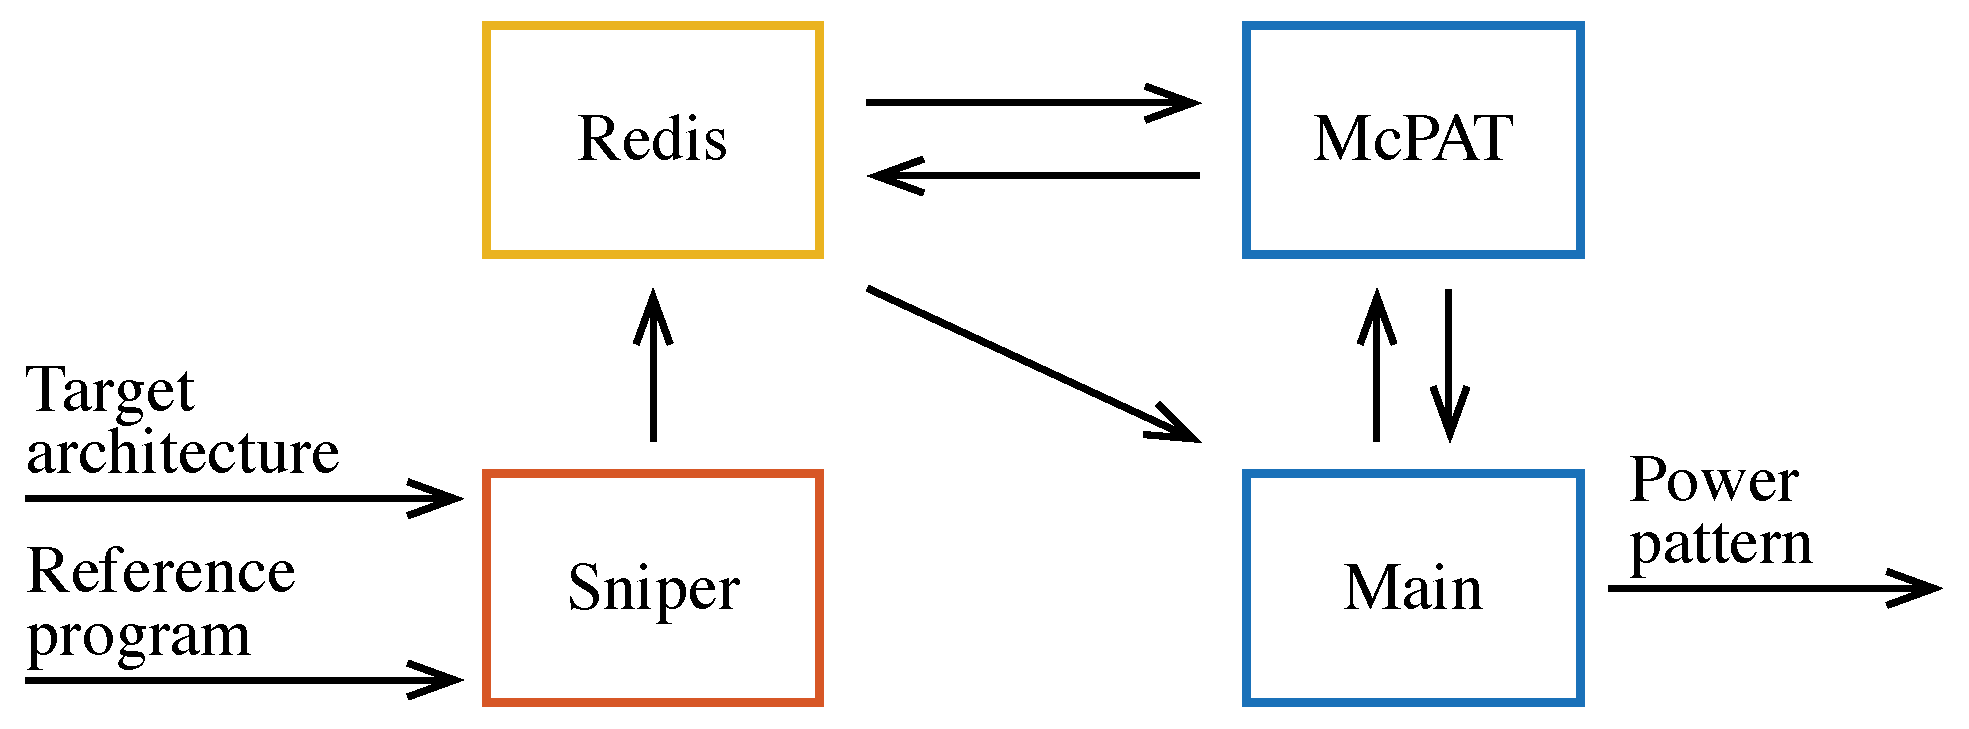
\includegraphics[width=1.0\columnwidth]{include/assets/figures/recorder.pdf}
  \caption{
    The recording infrastructure. The Recorder tool corresponds to the two blue
    boxes on the right-hand side of the figure.
  }
  \flab{recorder}
\end{figure}

\begin{table}
  \begin{threeparttable}
    \caption{Target architecture}
    \begin{tabular*}{\linewidth}{=L{70pt}l}
      \toprule
      Component    & Description \\
      \midrule
      Core         & 2660 MHz, 1.2 V \\
      L1-I/D cache & 32 KB, 4-way, LRU, private \\
      L2 cache     & 256 KB, 4-way, LRU, private \\
      L3 cache     & 8192 KB, 16-way, LRU, one per four cores \\
      \bottomrule
    \end{tabular*}
    \tlab{target}
    \begin{tablenotes}
      \item A detailed description of the target architecture can be found in
      the \texttt{nehalem.cfg} and \texttt{gainestown.cfg} configuration files
      of Sniper.
    \end{tablenotes}
  \end{threeparttable}
\end{table}
% vim: nowrap tw=0

As the name suggests, the purpose of \recorder\ is recording. More specifically,
the tool records reference workload patterns, which are needed as an input to
\streamer. The recording infrastructure is depicted in \fref{recorder}.

The performance simulator is Sniper \cite{carlson2011}.

The power simulator is \sc{McPAT} \cite{li2009}.

The key-value storage is Redis \cite{redis}.

The database is SQLite \cite{sqlite}.


\subsection{Streamer} \slab{streamer}
\begin{figure}
  \centering
  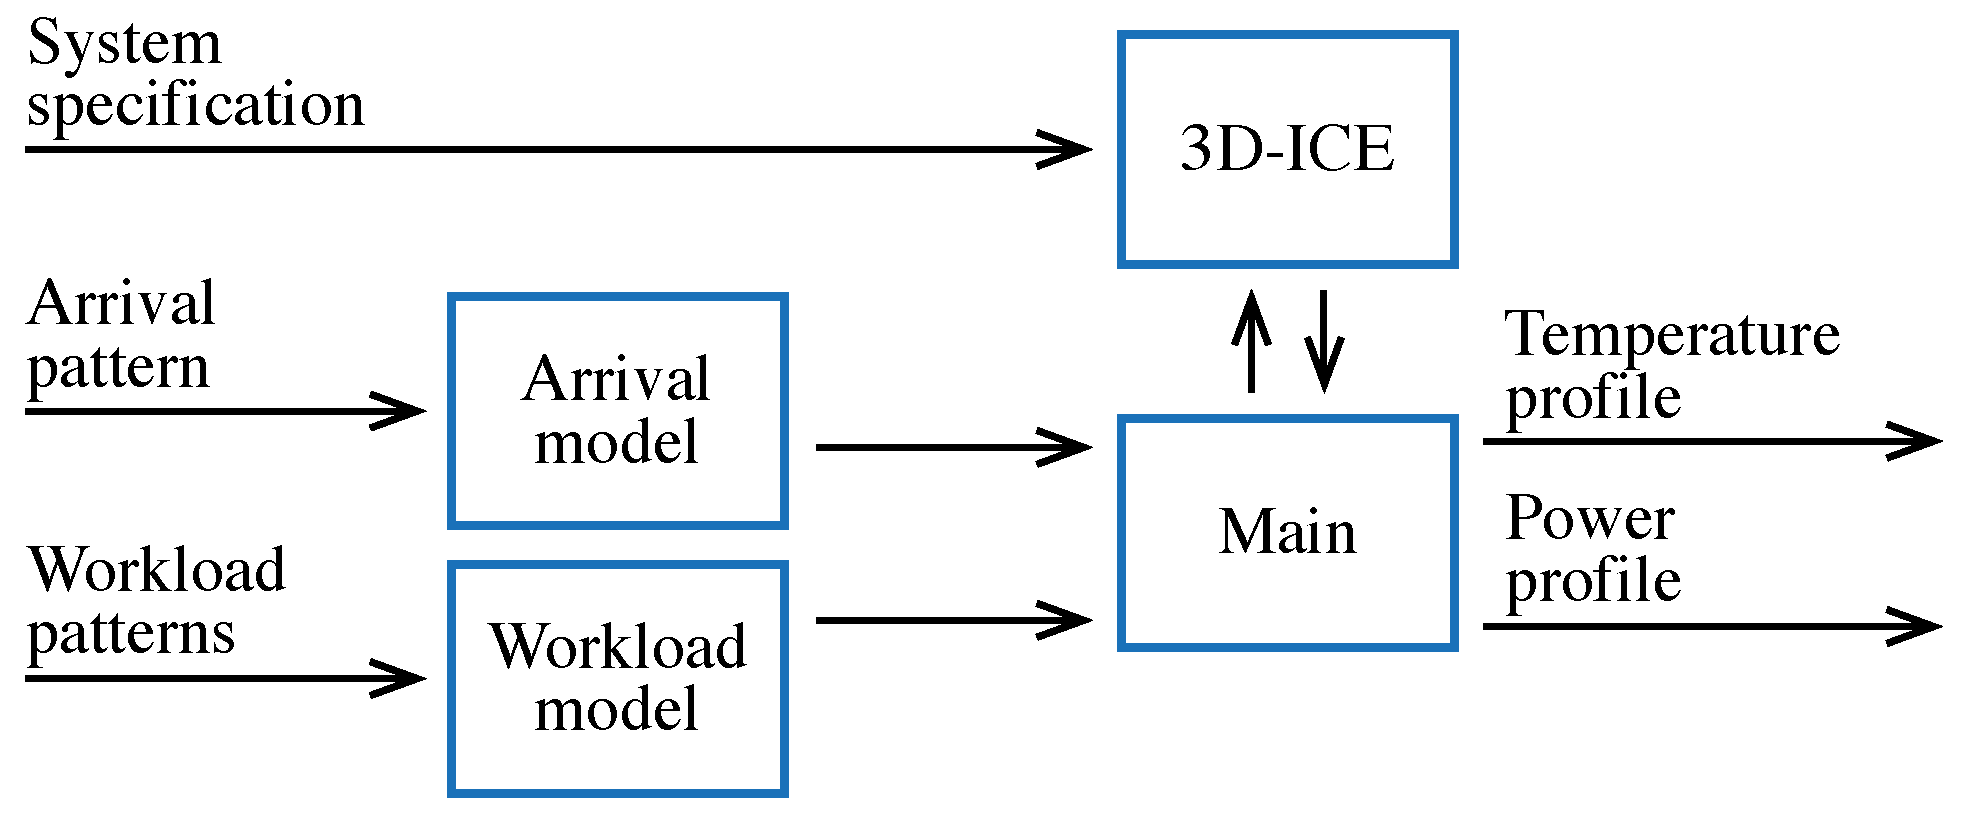
\includegraphics[width=1.0\columnwidth]{include/assets/figures/streamer.pdf}

  \caption{The Streamer tool. \emph{System specification} refers primarily to
  the information about the thermal package and floorplans of the platform,
  which are needed for temperature simulation. \emph{Job model} refers jointly
  to the traffic and workload models (\sref{traffic} and \sref{workload}).}

  \flab{streamer}
\end{figure}

The Streamer tool corresponds to the data-synthesis stage, which means that it
is responsible for synthesizing power and temperature data using reference data
as a material for the synthesis; see the module labeled ``Streamer'' in
\fref{methodology}. The structure of the tool is laid out in \fref{streamer}.

Given a traffic pattern and a set of workload patterns, Streamer proceeds as
follows. The traffic pattern is processed as it was described in \sref{traffic},
which results in an adequately configured multifractal wavelet model
\cite{riedi1999}. The model is then used to generate a stream of arrival times.
The arrival times are fleshed out using the workload patterns, which was
explained in \sref{workload}. The result is a stream of jobs, and the whole
operation is referred to as job modeling in \fref{streamer}. The rest follows
\sref{composition}. The job stream is handled by a scheduling policy; in
\fref{streamer}, this policy is a part of the Main module. As the incoming jobs
are being scheduled, the power profile of the system under consideration is
being constructed. The power profile is piped into a temperature simulator (to
be discussed below), which delivers a temperature profile. The continuity of the
process is worth noting: just as with arrival times and jobs, power and
temperature can be viewed as streams of data. The synthesized data (power and
temperature) can be fed back to the scheduler and/or stored for later usage. In
the latter case, similar to reference data, the output is an SQLite database.

Let us now outline how temperature simulation is undertaken inside Streamer. The
simulation is based on the popular thermal \sc{RC} model. In this paradigm, a
so-called thermal \sc{RC} circuit representing the system at hand is constructed
and then used to analyze the thermal behavior of the system. The analysis boils
down to solving a system of differential equations, which can be done using
different integration techniques. In our case, the solution is based on a solver
leveraging exponential integrators \cite{hochbruck2010, ukhov2014}. The
construction of thermal circuits is outsourced to either HotSpot
\cite{skadron2004} or \sc{3D-ICE} \cite{sridhar2010} (see \fref{streamer}). Both
simulators are based on the thermal \sc{RC} model, and we extract the circuits
that they build, which results in a unified interface for working with the two
alternatives.

To summarize this subsection, the Streamer tool produces streams of power and
temperature data, and this procedure closely follows the ideas presented in
\sref{methodology}. Our temperature simulation is based on the thermal \sc{RC}
model, in which thermal circuits are constructed by either HotSpot or
\sc{3D-ICE}.


In the conclusion of this section, we would like to make a number of general
comments about the toolbox. First, as mentioned earlier, our tools are composed
of a number of packages, and we pursued a clear separation of the
responsibilities of these packages. As a result, the packages can be swapped out
or reused in other contexts. Second, we also provide auxiliary scripts and tools
(for instance, a tool for constructing die floorplans based on the information
from \sc{McPAT}), which are not elaborated on here but available as a part of
the toolchain. Last but not least, the toolbox is open source \cite{sources},
and any feedback and contribution will be very much appreciated.
